% !TEX root = guia.tex

\chapter{tkz-euclide}
Tikz es un paquete bastante robusto, capaz de hacer casi cualquier imagen que queramos. La parte básica es simple, pero al avanzar más se requieren más conocimientos del lenguaje (pgf en este caso) y matemáticos. Hacer geometría euclidiana es un ejemplo donde se necestian las dos hábilidades mencionas, así que tener una libreria que hace los cálculos por nosotros y facilita la sintaxis es una buena idea.

Ahora veremos algunas construcciones básicas hechas con \texttt{tkz-euclide}. Lo primero es cargar el paquete, en este caso sólo es posible hacerlo como un paquete y no como una libreria de \texttt{tikz}.
\begin{verbatim}
  \usepackage{tkz-euclide}
\end{verbatim}

Lo más básico es cómo poner puntos, segmentos, y algunas figuras, por ejemplo

\begin{minipage}{0.4\linewidth}
  \begin{verbatim}
    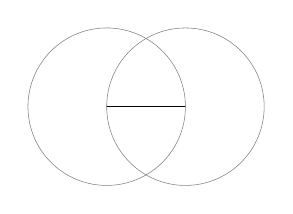
\begin{tikzpicture}
      \tkzDefPoint(0,0){A}
      \tkzDefPoint(1,0){B}
      \tkzDrawSegment(A,B)
      \tkzDrawCircles(A,B B,A)
    \end{tikzpicture}
  \end{verbatim}
\end{minipage}\hspace{1cm}
\begin{minipage}{0.5\linewidth}
  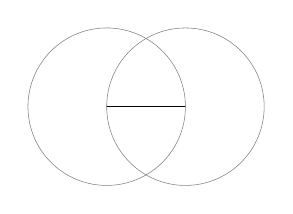
\begin{tikzpicture}
    \tkzDefPoint(0,0){A}
    \tkzDefPoint(1,0){B}
    \tkzDrawSegment(A,B)
    \tkzDrawCircles(A,B B,A)
  \end{tikzpicture}
\end{minipage}

En este ejemplo podemos notar que usamos un comando en singular para poner los puntos \(A\) y \(B\) y una versión en plural para los circulos. En este último el primer circulo tiene centro en \(A\) y radio \(AB\), análogamente el segundo. Además, cada circulo está separado por un espacio.

En \texttt{tkz-euclide} casi cada comando tiene una versión en singular y una en plural. El ejemplo anterior todavía no es muy bueno ya que todos los puntos los estamos poniendo manualmente por medio de coordenadas. Veamos una modificación del ejemplo donde se obtenga algún punto por medio de un cálculo hecho por \texttt{tkz-euclide}

\begin{minipage}{0.4\linewidth}
  \begin{verbatim}
    \begin{tikzpicture}
      \tkzDefPoints{0/0/A, 2/0/B}
      \tkzInterCC(A,B)(B,A)
      \tkzGetPoints{C}{D}
      \tkzDefMidPoint(A,B)
      \tkzGetPoint{M}
      \tkzDrawPoints(A,...,D)
      \tkzDrawSegments(A,B M,D)
      \tkzDrawCircles(A,B B,A)
      \tkzLabelPoints(A,B,D)
      \tkzLabelPoint[above](C)
    \end{tikzpicture}
  \end{verbatim}
\end{minipage}\hspace{1cm}
\begin{minipage}{0.5\linewidth}
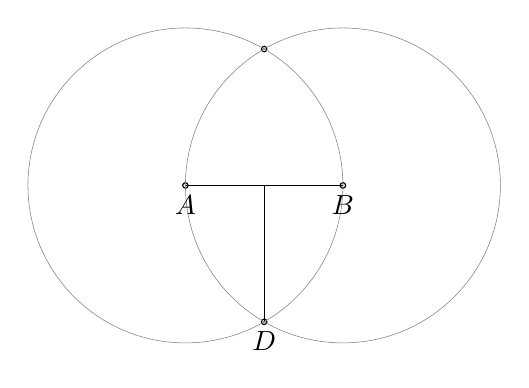
\begin{tikzpicture}
  \tkzDefPoints{0/0/A, 2/0/B}
  \tkzInterCC(A,B)(B,A)
  \tkzGetPoints{C}{D}
  \tkzDefMidPoint(A,B)
  \tkzGetPoint{M}
  \tkzDrawPoints(A,...,D)
  \tkzDrawSegments(A,B M,D)
  \tkzDrawCircles(A,B B,A)
  \tkzLabelPoints(A,B,D)
\end{tikzpicture}
\end{minipage}
